\documentclass{article}
\usepackage{graphicx} % Required for inserting images
\usepackage{hyperref}
\usepackage{cite}
\usepackage{float}

\title{Practical 1- Research Assignment}
\author{Hayley Dodkins u21528790}
\date{18 February 2025}

\begin{document}
\maketitle

\section{}
Esoteric programming languages also known as esolangs are designed to be unconventional. They can be categorised into the following types: 
\begin{itemize}
    \item Objective-Driven Languages: These languages were designed to achieve an objective such as producing as few instructions as possible or languages to be used in code golf where the goal is to have the shortest source code to solve a given algorithm \cite{Tomassetti, Stuart}.
\end{itemize}
\begin{itemize}
    \item Unusable languages: Designed to be intentionally difficult to write. These languages often restrict the use of symbols. A well-known example would be a language called Brainfuck which consists of only 8 commands \cite{Tomassetti}.
Concept-exploration languages introduce new programming concepts. Befunge arranges code in a two-dimensional grid allowing execution in multiple directions \cite{Tomassetti}.
\end{itemize}
\begin{itemize}
    \item Artistic languages: These languages are designed to resemble something other than traditional programming source code. For instance, Piet is a language designed to look like abstract art, while Shakespeare is a language that emulates the style of Shakespearean play \cite{Stuart}.
\end{itemize}
\begin{itemize}
    \item Joke languages: Created for humour. INTERCAL was a language designed that requires the programmer to use the keyword “please” an appropriate number of times, if not used enough the compiler deems the code impolite, if used too much the programmer is overly ingratiating \cite{Elvis}.
\end{itemize}

\section{}
\subsection{Funges}
Funges are difficult to compile. The compiler cannot perform a static analysis and determine the control flow of a program and, due to the self-modifying behaviour, it is hard for the compiler to make any traditional modifications \cite{Oak, Ohms}.
Funges enable a way to explore alternative computation models different to the classic Von Neumann architecture where there is linear instruction execution, Funges explore the idea of multi-dimensional computing and non-traditional execution flows \cite{Morr}.
\subsection{Turing Tarpits}
Turing tarpits are considered Turing complete, meaning that theoretically the language can be used to solve any computational problem given enough memory and time \cite{Harrison}. Turing tarpits are considered practically unusable because they are often difficult to write due to only using a limited number of symbols \cite{Tomassetti}.

\section{}
\subsection{INTERCAL}
\textbf{Year of Initial Design:} 1972\\
\textbf{Designers:} Donal R. Woods and James M Lyon\\

\textbf{General Characteristics:}
The goal of INTERCAL was to be a compiler language with nothing in common with any other major language at the time. The full name of the language is "Compiler Language With No Pronounceable Acronym", which is abbreviated to "INTERCAL" \cite{Woods}. 

\textbf{Variable Types:}
INTERCAL has five types of variables \cite{EsolangsINTERCAL}:
\begin{itemize}
    \item The 16-bit unsigned integer (.) followed by a number
\end{itemize}
\begin{itemize}
    \item The 32-bit unsigned integer (:) followed by a number
\end{itemize}
\begin{itemize}
    \item The array of 16-bit unsigned integers (,) followed by a number
\end{itemize}
\begin{itemize}
    \item The array of 32-bit unsigned integers (;) followed by a number
\end{itemize}
\begin{itemize}
    \item Constants are 16-bit unsigned integers (#) followed by a number
\end{itemize}

\textbf{Operators:}
INTERCAL has 5 operators, two binary operators and three unary operators \cite{Woods}. 
\begin{itemize}
    \item Interleave (¢): A binary operator that takes two 16-bit values and produces a 32-bit result by alternating the bits of the operands.
\end{itemize}
\begin{itemize}
    \item Select(~): Extracts bits from one operand based on the second operand’s 1-bits. 
\end{itemize}
\begin{itemize}
    \item The unary operators: & (logical AND), V (logical OR), and V− (logical XOR).
\end{itemize}

\textbf{Syntax}
\begin{itemize}
    \item INTERCAL consists of a list of statements preceded by an optional line label followed by DO, PLEASE, or PLEASE DO \cite{Woods}.  
\end{itemize}
\begin{itemize}
    \item INTERCAL enforces a ''politeness rule'', where 1/3 to 1/5 of statements must include "PLEASE." If too few or too many of the statements are polite, the compiler will reject the program \cite{Woods}.
\end{itemize}
\begin{itemize}
    \item The angle (<) followed by a worm (-) is the equivalent of the assignment operator (=) in FORTRAN \cite{Woods}.
\end{itemize}
\begin{itemize}
    \item The NEXT statement is used for subroutine calls and unconditional transfers where DO (label) NEXT and PLEASE DO (label) NEXT are the two forms of this statement \cite{Woods}.
\end{itemize}
\begin{itemize}
    \item The statement PLEASE FORGET exp, causes the expression to be evaluated, and the specified number of entries to be removed from the stack \cite{Woods}. 
\end{itemize}
\begin{itemize}
    \item PLEASE GIVE UP is used to exit from a program \cite{Woods}. 
\end{itemize}
\begin{itemize}
    \item Input is taken with the statement DO WRITE IN x, where x would be a variable \cite{Woods}.
\end{itemize}
\begin{itemize}
    \item INTERCAL does not have an equivalent to an IF statement or GO TO, instead DO ABSTAIN FROM and PLEASE ABSTAIN FROM is used to ignore all statements of specified types \cite{Woods}.
\end{itemize}
\cite{Woods}
\begin{figure}[H]
    \centering
    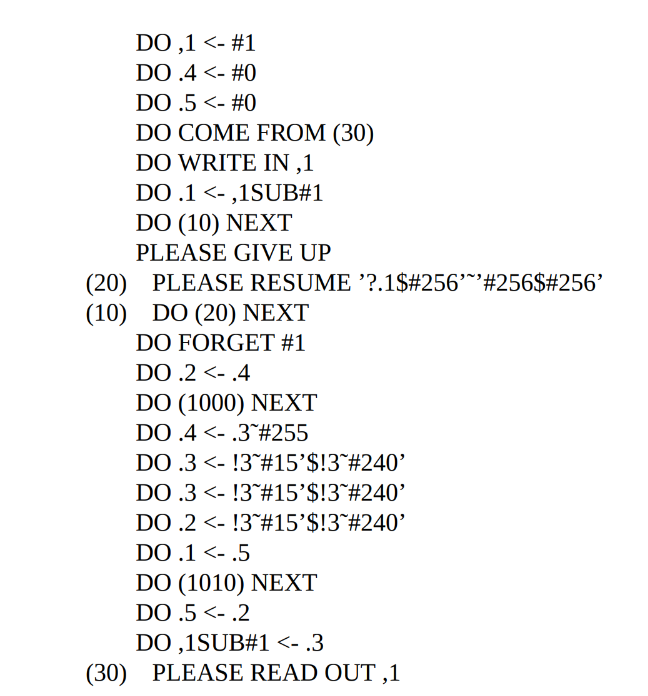
\includegraphics[width=0.5\linewidth]{Screenshot From 2025-02-18 08-57-51.png}
    \caption{This example code was taken from \cite{Woods}.}
\end{figure}


\subsection{Piet}
\textbf{Year of Initial Design:} 2001\\
\textbf{Designers:} David Morgan-Mar\\
Piet is a visual esoteric programming language in which programs resemble abstract paintings inspired by Piet Mondrian \cite{EsolangsPiet}. The program execution follows a direction pointer that moves across coloured blocks (codels), interpreting colour transitions as commands \cite{MorganMar}. 

\textbf{Data handling:}  
Piet is stack-based using only integer values \cite{MorganMar}.

\textbf{Tokens:}
\begin{itemize}
    \item The smallest entity is a codel which consists of a single pixel or many pixels depending on the size of the image \cite{Moosleitner}.
\end{itemize}
\begin{itemize}
    \item A colour block is a continuous block of codels of the same colour \cite{Moosleitner}.
\end{itemize}

\textbf{Program traversal:} 
    \begin{itemize}
        \item An interpreter starts at the top left codel (this codel cannot be black). The interpreter moves from one colour block to another using the direction pointer and codel chooser to decide which colour block is next \cite{Moosleitner}.
    \end{itemize}
    \begin{itemize}
        \item The direction pointer can move in four directions, up, down, left or right. This pointer initially points right \cite{Moosleitner}.
    \end{itemize}
    \begin{itemize}
        \item The codel chooser can point left or right. At the start the codel chooser points to the left. The interpreter uses the codel chooser to choose which one of the neighbouring colour blocks along the border is the next one to move into \cite{Moosleitner}.
    \end{itemize}
    \begin{itemize}
        \item The edges of a program and black colour blocks cannot be penetrated and limit possible movement options \cite{Moosleitner}.
    \end{itemize}
    \begin{itemize}
        \item If the interpreter moves into a white colour block, it follows the current direction of the direction pointer until a colour block is reached or a black colour block or edge is found \cite{Moosleitner}.
    \end{itemize}

\textbf{Colour-based Commands:}
\begin{itemize}
    \item When the interpreter moves from one colour block to the next one. It triggers the execution of commands \cite{Moosleitner}.
\end{itemize}
\begin{itemize}
    \item Commands are encoded in the amount of steps taken in hue and lightness of the colour transition \cite{Moosleitner}.
\end{itemize}
\begin{itemize}
    \item Depending on the command executed an integer is either pushed onto the stack or popped off the stack \cite{Moosleitner}.
\end{itemize}

\begin{figure}[H]
    \centering
    
\includegraphics[width=0.5\linewidth]{Piet_hello_big.png}
    \caption{Taken from \cite{MorganMar}, the example Piet code above prints "Hello world!" and then exits.}
\end{figure}


\section{}
Design by contract (Dbc) is a software design approach where contracts (interaction protocols) are used to assert how classes and methods should interact. Dbc is achieved through the following concepts \cite{Nicolette}:
\begin{itemize}
    \item \textbf{Preconditions:} Assertions that must be true when a function is called \cite{Kaushik}.
\end{itemize}
\begin{itemize}
    \item \textbf{Postconditions:} Assertions that hold true once a function has been completed \cite{Kaushik}.
\end{itemize}
\begin{itemize}
    \item \textbf{Invariants:} Classes or properties that should remain unchanged when there is interaction between participants \cite{Kaushik}.
\end{itemize}

Both Clojure and Ada have native support for Design by contract \cite{DesignByContractWiki}.


\section{}
“Vibe programming” refers to a programming approach where developers rely heavily on AI coding tools to generate and debug code without deep understanding or analysis. When the AI tools fail, the developer results to random fixes until something works rather than systematically debugging the code.

\begin{itemize}
    \item \textbf{No critical thinking:} The developer does not engage in problem-solving but instead depends on AI-generated solutions. This reduces their ability to evaluate, debug or optimize code independently. Without the necessary critical thinking skills, developers cannot fix issues which will lead to inefficiencies when AI tools are not available or produce suboptimal solutions.
\end{itemize}
\begin{itemize}
    \item \textbf{Lack of innovation:} AI is trained on existing code, meaning AI generates standard and widely used solutions rather than optimized more advanced approaches. This could stifle innovation, as AI would favour well-known solutions over new languages, frameworks or methodologies making it difficult for emerging technologies to gain traction.
\end{itemize}
\begin{itemize}
    \item \textbf{Reliance on AI Tools:} If developers rely entirely on AI tools for coding, any downtime,  outage or limitation can render them unable to do their job. They would struggle to understand the AI-generated code or any error messages. This type of dependence creates a fragile workflow where productivity is tied to the availability of  AI-tools rather than the programmer’s skill set. 
\end{itemize}
\begin{itemize}
    \item \textbf{Lack of programming knowledge:} A developer who only codes through the use of AI assistance may never gain a deep understanding of programming languages and their features. Since AI-generated code is based on common patterns the developer will never learn how to use more advanced features. These developers would struggle to assess if a piece of code is truly good or just good enough as they lack the foundational knowledge.
\end{itemize}

\bibliographystyle{plain}
\bibliography{references}
\end{document}
